\chapter{A semi-empirical model point of view} \label{ch:SEM}

%\begin{center}
%  {\it ``If could add an introductionary text here.''}
%  \vspace{1cm}
%\end{center}

\begin{center}
  {\it The work in this chapter has been submitted for publication on the main journal of the Monthly Notices of the Royal Astronomical Society.}
  \vspace{1cm}
\end{center}

In this Chapter we aim to expand the results from Chapter \ref{ch:observations} and understand how they originate by taking advantage of semi-empirical models (SEMs) and the sample selected in there.

Semi-empirical models are a competitive, fast and flexible methodology, extensively used in recent years to constrain the degree of evolution and mergers in galaxies, as well as the degree of coevolution with their central BHs \citep{2013ApJ...762...70C, 2019MNRAS.487..275G, 2019MNRAS.487.2005C, 2020arXiv201002957A, ShankarNat, Allevato21}. 
It is particularly relevant the application of SEMs to the creation of active and normal galaxy ``mock'' catalogs \citep[e.g.][]{2019MNRAS.487..275G, 2019MNRAS.487.2005C, 2020arXiv201002957A, ShankarNat, Allevato21},
which are a vital component of the planning of imminent
extra-galactic surveys such as Euclid \citep[][]{laureijs11}.
The advantage of this methodology is that by using few input relations, 
it creates a mock catalog of active and normal galaxies that – by design – reproduces 
the X-ray luminosity function of active galaxies. 
Moreover, these models allow us to disentangle the effects on 
relevant relations of the input parameters,
shedding light on the processes controlling the co-evolution of BHs and their hosts.

In this Chapter we perform new estimates for the X-ray detected sample selected in Chapter~\ref{ch:observations} and use comprehensive semi-empirical mock 
catalogs of active BHs 
to pin down which parameters control the shape and evolution of the \LXMS\ relation. We explore a variety of inputs in our model, such as the shape of the Eddington ratio distribution $P(\log\lambda)$ which carries information on the accretion of a BH, or the normalization of the \MBHMS\ scaling relation. More specifically, we find that its slope and normalization are mostly determined by, respectively, the M$_{\rm BH}-{\rm M}_*$ relation and mean Eddington ratio.

In Section~\ref{sec:model} we present our model and in Section~\ref{sec:results} we highlight the main parameters controlling the L$_{\rm X}-{\rm M}_*$ evolution at different redshifts and galaxy phases.
In Sections~\ref{sec:disc}, and~\ref{sec:concl} we discuss our findings and draw our conclusions on their relevance to the galaxy-BH co-evolution.

\section{Building robust AGN mock catalogs}\label{sec:model}
In this study we create realistic mock catalogs of AGN and non-active galaxies to study which input parameters mostly control the \LXMS{} relation at different redshifts. Below provide the most relevant steps in the generation of our mocks, and refer the reader to \citet{Allevato21} where the model is presented, for full details. In the work in this Chapter we run the model testing and tuning the entire range of input parameters. We also perform the analysis of the model output, the galaxy mock catalogs, in order to be able to compare the mocks to our observables.

The first step for the creation of mocks consists in generating a halo distribution via a halo mass function from \citet{2008ApJ...688..709T} at the redshift of interest. To each dark matter halo we assign a galaxy stellar mass via abundance matching techniques \footnote{We immediately note that the exact choices for this first step of the mock generation are irrelevant to our results and conclusions discussed below. As in this work we are not studying the environment of active galaxies, the information on host halo mass is here only given for completeness. Equivalent mocks could be generated by simply extracting galaxies from an input stellar mass function.}, using the relation of \citet[][]{moster10} with updated parameters from \citet[][Eq.~5]{2019MNRAS.483.2506G} with a normal scatter in stellar mass at fixed halo mass of $0.11$~dex.
We then assign a BH mass via the empirically calibrated \MBHMS\ relation by \citet{2015ApJ...813...82R}, with an intrinsic scatter of $0.55$ dex, and also explore the impact of adopting other M$_{\rm BH}-{\rm M}_*$ relations from \citet{2016MNRAS.460.3119S}, \citet{2018ApJ...869..113D} and \citet{2019ApJ...876..155S}, which bracket the systematic uncertainties in the BH-galaxy stellar mass in the local Universe. 
We then assume that each relation does not evolve with redshift, as suggested by a number of studies \citep[e.g.][and Fig.~\ref{fig:comp_models}]{shankar09c,2019ApJ...885L..36D, 2020ApJ...889...32S, 2020MNRAS.493.1500S}.
To each galaxy and BH we then assign an Eddington ratio $\lambda\equiv L_{bol}/L_{\rm Edd}$ and convert bolometric luminosities $L_{bol}$ to intrinsic (i.e., unobscured) 2-10 keV X-ray luminosities $L_X$ via the same bolometric corrections $k_X$ adopted in Chapter~\ref{ch:observations} (see Sec.~\ref{subsec:LX_BHAR}). Following the formalism in, e.g., \citet{Shankar13Acc} and \citet{Allevato21} and references therein, which in turn follows the one routinely adopted in continuity equation models, the AGN luminosity function at any given redshift $z$ can be expressed by the convolution
\begin{equation}
\Phi(\log L_{bol},z)=\int_{\log \lambda_{\rm min}}^{\log \lambda_{\rm max}}U(y,z) n(y,z) P(\log \lambda,z)d\log \lambda \, 
\label{eq:PhiL}
\end{equation}
where $y=\log {\rm M}_{\rm BH}$ and $n(y,z)$ is the total BH mass function. \PLz\ is the
Eddington ratio distribution, which we assume for simplicity to be independent of BH mass,
normalized to unity in the range $\log \lambda_{\rm min}<\log \lambda<\log \lambda_{\rm max}$.
$U(y,z)$ is the \emph{intrinsic} duty cycle, i.e., the fraction of all black holes of mass $y$
that are active and accreting mass at an Eddington rate in the range
$\log \lambda_{\rm min}<\log \lambda<\log \lambda_{\rm max}$ at redshift $z$.
We set our minimum Eddington ratio to $\log \lambda_{\rm min}=-4$ and the maximum
Eddington ratio to $\log \lambda_{\rm max}=1$, noticing that the exact value chosen for
$\log \lambda_{\rm max}$ does not alter any of our results as the adopted Eddington ratio
distributions have extremely low probabilities above the Eddington limit.

The flexibility offered by Eq.~\ref{eq:PhiL} allows to disentangle the effects of the shape
of \PLz, which carries information on the accretion properties of a BH, from the fraction
$U(y,z)$ of active BHs accreting above a certain threshold in Eddington ratio. The reference
$P(\log \lambda,z)$ distribution is taken to be a simple Gaussian in $\log \lambda$
characterized by a standard deviation $\sigma$ and a mean $\mu$. We will show that the shape
of the \PLz\ distribution plays a minor role in the outputs as long as the characteristic
Eddington ratio, defined as
\begin{equation}
\zeta_c(z)\equiv\left<\log \lambda\right>(z)=\int_{\log\lambda_{\rm min}}^{\log \lambda_{\rm max}} P(\log\lambda,z)\log(\lambda) \,d\log(\lambda)\, ,
\label{eq:zeta_c}
\end{equation}
is the same. In Eq.~\ref{eq:zeta_c} $\log\lambda_{L_{\rm X,min}}$ is the Eddington ratio corresponding to the limiting luminosity at that redshift.
We assume a constant duty cycle of $U=0.2$ as suggested by \citet{goulding10} from local X-ray
AGN, but we also explore the impact on our results of varying the input duty cycle with
BH mass, specifically decreasing with M$_{\rm BH}$ as inferred by \citet{2010A&A...516A..87S}
and \citet{2015MNRAS.447.2085S}, and also increasing with M$_{\rm BH}$, as proposed by
\citet{2019MNRAS.488...89M}. Although these works were based on AGN samples with different
selections, we use these duty cycles simply as a guidance to explore the impact on our results
of different ``shapes'' of the input intrinsic duty cycles $U(y,z)$.

When comparing with the data we must retain from the full BH mock only those active BHs shining above the X-ray flux limit of the observational survey \citep[e.g.,][]{Shankar13Acc}. In our reference sample, the \textit{Chandra} COSMOS Legacy Survey \citep[COSMOS-Legacy,][]{2016ApJ...819...62C}, the X-ray flux limit corresponds to luminosities of $L_X=10^{42}\, {\rm erg/s}$ in the lower redshift bin ($z=0.45$), increasing by an order of magnitude or more at higher redshifts (see below for details). When computing all AGN-related observational probes, such as the AGN luminosity function (Eq.~\ref{eq:PhiL}), the characteristic Eddington ratio $\zeta_c(z)$ (Eq.~\ref{eq:zeta_c}), or the mean X-ray luminosity (Eq.~\ref{eq:meanLx}), we thus include only those active black holes shining above the \textit{Chandra} COSMOS Legacy Survey flux limit at the given redshift{\footnote{The COSMOS field is a great combination of area and depth making it ideally suited to probe the accretion properties of active BHs. A deeper field may be more sensitive to the faint end shape of the Eddington ratio distribution, but would not allow to include more luminous sources. A shallower field on the other hand, may return better statistics for the more luminous sources, but rapidly losing the fainter ones.}}. For example, although we fix our minimum Eddington ratio to $\log \lambda_{\rm min}=-4$ for our input \PLz\ (e.g., in Eq.~\ref{eq:PhiL}), after imposing the cut in X-ray flux limit, among the BHs with mass ${\rm M}_{\rm BH} \lesssim 10^8\, M_{\odot}$ in the lowest redshift bin, only those accreting at an Eddington rate $\log \lambda_{\rm X, min} \gtrsim -3$ will be included in the comparison with the data. We will discuss below that the flux limit plays a non-negligible role when comparing theoretical AGN mocks to observations, particularly with respect to the observed fraction of active black holes as a function of host galaxy stellar mass (Figure~\ref{fig:AGN_fractions}).

We assign SFRs to quiescent, normal star-forming, and starburst galaxies based on their respective SFR-M$_*$ relation.
For starburst and quiescent galaxies, we adopt the SFR fits from Table~\ref{table:all_fitpar},
while for the ``main sequence'' we adopt the 
\citet[Eq.~9]{2015A&A...575A..74S} flexible parametric formula
\begin{equation}
    \log_{10}\left(\frac{\rm SFR}{M_\odot yr^{-1}}\right)= m - m_0 +a_0 r - a_1[\max(0,m-m_1-a_2r)]^2
	\label{eq:SFR}
\end{equation}
with $m\equiv\log_{10}(M_*)-9$ and $r\equiv\log_{10}(z+1)$. Best-fit parameters for our COSMOS data are $a_0=2.29\pm 0.12$, $a_1=0.25 \pm 0.04$, $a_2=0.33 \pm 0.30$, $m_0=0.64 \pm 0.03$, $m_1=0.55\pm 0.11$, and the fit is shown in Fig.~\ref{fig:SFR_2D_fit}. We add a dispersion of $0.2$~dex to the SFR. 
\begin{figure*}
%%%%%\vspace{8cm}
\begin{center}
  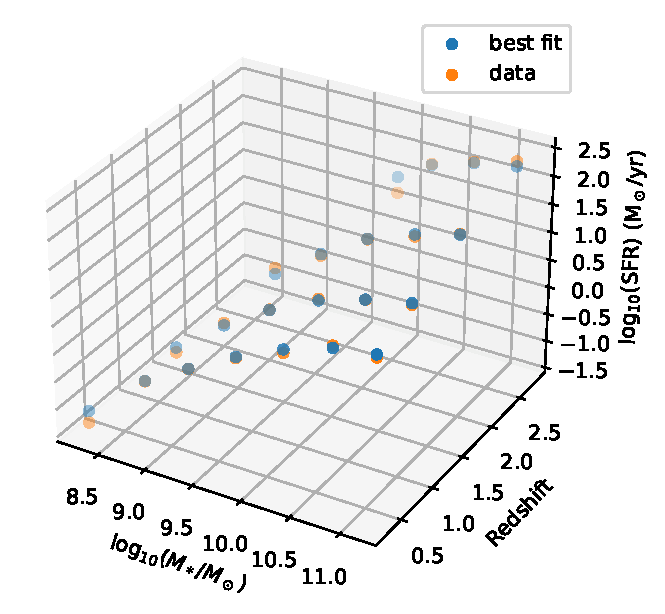
\includegraphics[width=0.65\linewidth]{Figs/Chapter3/2D_SFR_fit_data.pdf}
  \caption{A 2-dimensional plot of the SFR data for star forming galaxies from Chapter~\ref{ch:observations} as a function of ${\rm M}_*$ and redshift, compared with our best fit of Eq.~\ref{eq:SFR}.
  }
    \label{fig:SFR_2D_fit}
\end{center}
\end{figure*}

\begin{figure*}
%%%%%\vspace{8cm}
\begin{center}
  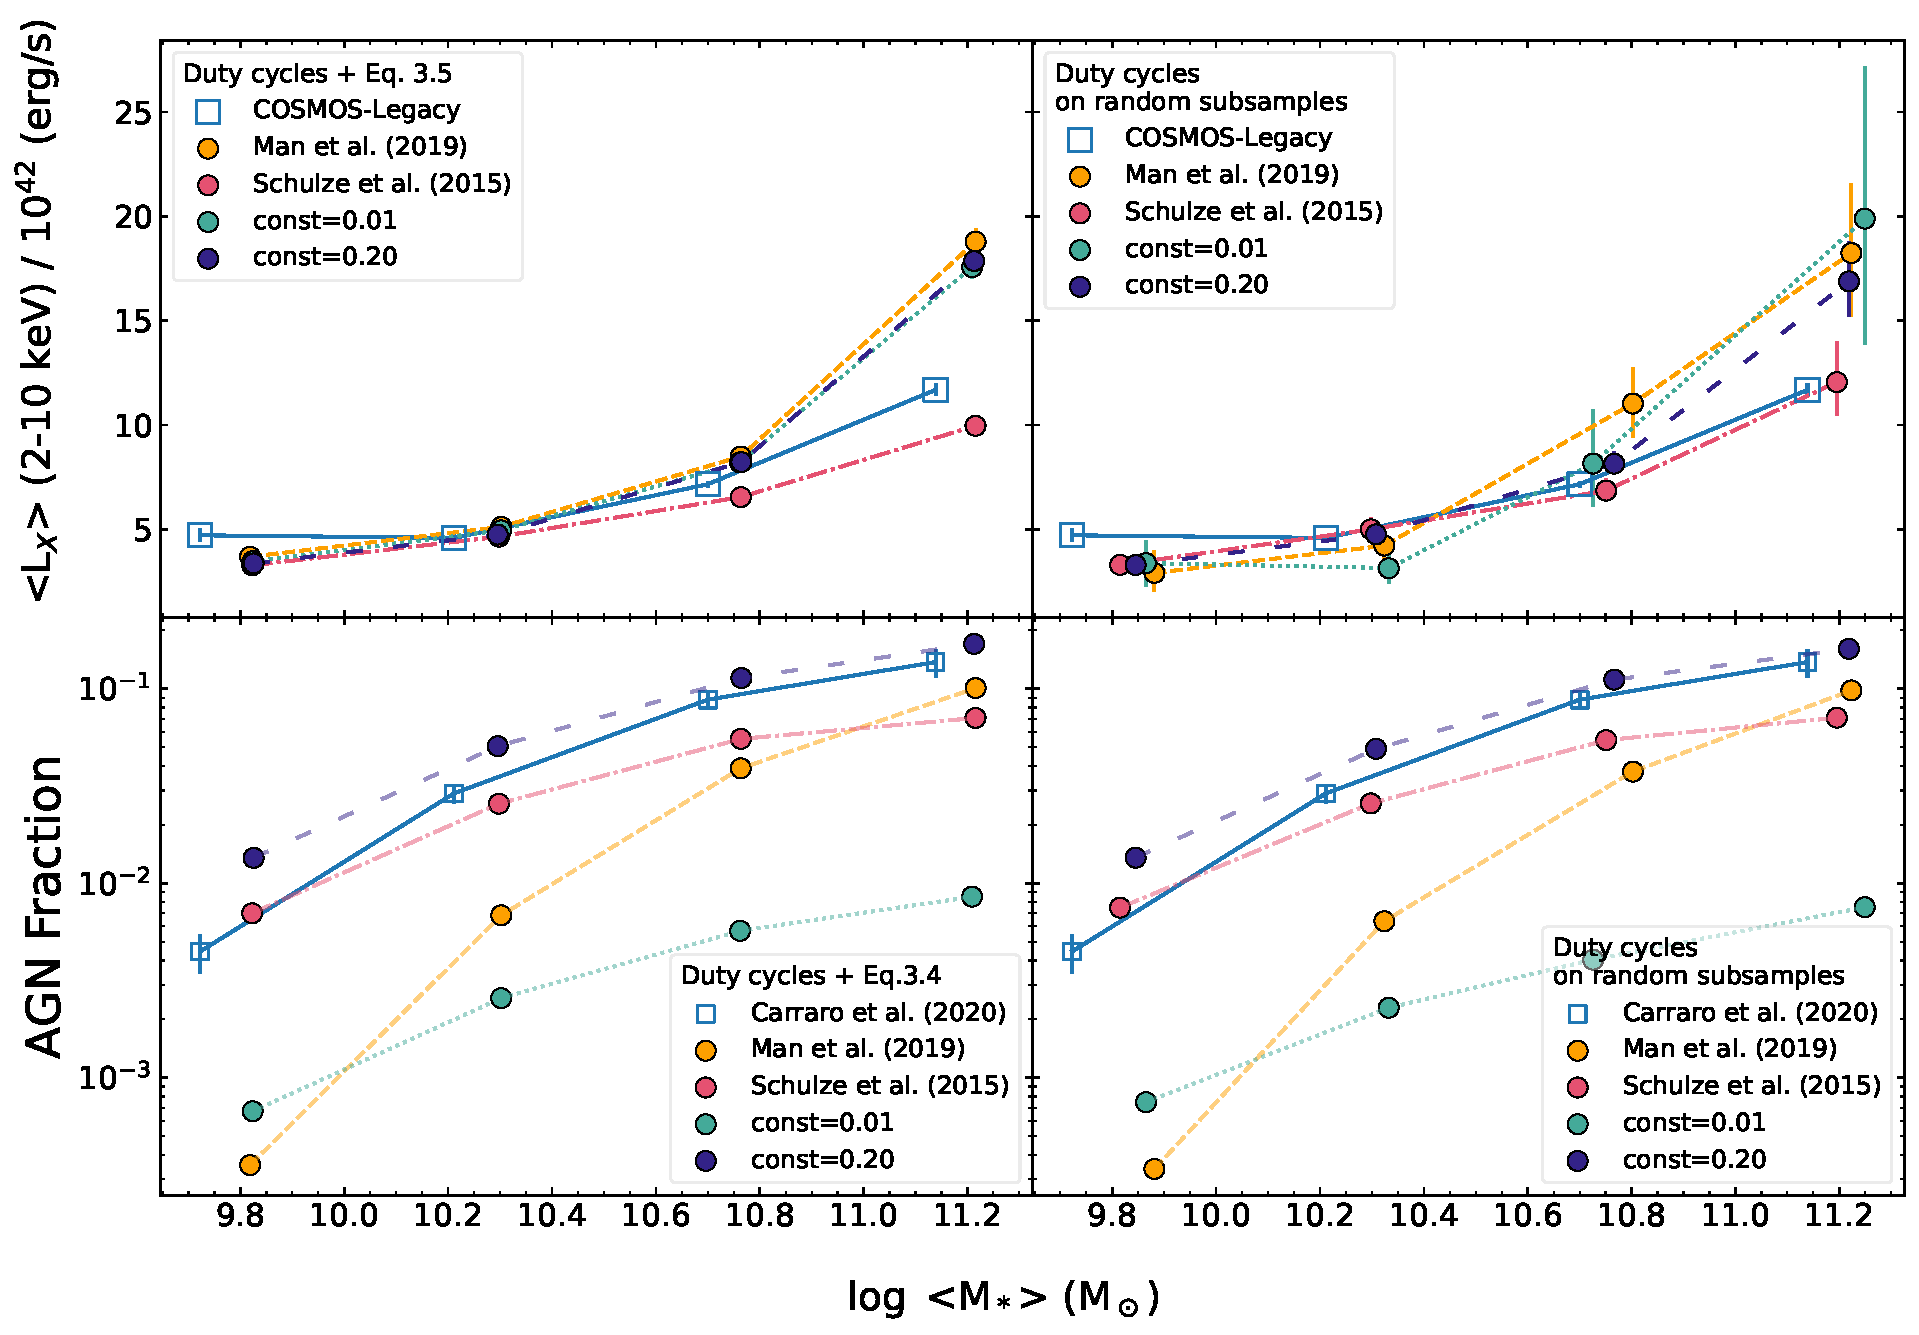
\includegraphics[width=\linewidth]{Figs/Chapter3/test_mean_subsamples.pdf}
  \caption{Comparison of \LX{} and AGN fraction obtained with various input duty cycles as in our approach in the rest of the Chapter (left panels, using Equations~\ref{eq:AGN_fraction}, and~\ref{eq:meanLx}) and by randomly assigning a star formation category and AGN activity flag.
  }
    \label{fig:test_subsamples}
\end{center}
\end{figure*}

Irrespective of their duty cycle, we assign to each galaxy in the mock an X-ray luminosity
from X-ray binary emission following \citet[][Table 3]{2016ApJ...825....7L}, and
when computing the average X-ray luminosity competing to a given bin of stellar mass, we then
subtract the mean binary emission competing to that bin of stellar mass and star formation rate
as in Sec.~\ref{subsec:LX_BHAR}.
We note that neglecting X-ray binary emission entirely from our procedure would yield very
similar results.
Following the procedure described above, we generate diverse galaxy mock catalogs with
distinct choices of the input \MBHMS{} scaling relations, duty cycles, and $P(\log\lambda,z)$
distributions. 
We then divide each AGN mock catalog in bins of stellar mass, and select the
BHs that shine above the flux limit of the COSMOS-Legacy survey \citep{2016ApJ...817...34M},
i.e., the ``detected'' sources of the mock, as discussed above. The first observable we
compute is the AGN fraction, defined as
\begin{equation}
{\rm AGN\;fraction}(M_*,z)=\frac{\sum_i U_{i,{\rm detected}}} {N_{\rm tot}}\, ,
    \label{eq:AGN_fraction}
\end{equation}
where the sum in the numerator runs over all active BHs above the flux limit, and $N_{\rm tot}$
at the denominator is the total number of active and normal galaxies in
the specified stellar mass bin. We note that the probability for a galaxy to be detected above
a certain X-ray luminosity threshold, i.e., the ``observed'' duty cycle, will depend not only
on the assumed (intrinsic) duty cycle, but also on other properties such as its BH mass and
Eddington ratio. We will discuss below the differences between observed and intrinsic duty
cycles and highlight how different input parameters in the mocks can generate similar observed
fractions of AGN.
The comparison between the observed AGN fraction and predicted input duty cycle \UMBHz\ yields important constraints on the accretion properties of active BHs when coupled to other observables, as we will discuss below.
Finally, we perform 500 bootstraps out of which we extract the median SFR and M$_*$, and the linear mean L$_{\rm X}$ weighted by the AGN duty cycle %\log M_{BH,i}
\begin{equation}
\left<L_X\right>=\frac{\sum_i U_i(y_i,z) L_X(y_i)} {\sum_i U_i(y_i,z)}\, ,
    \label{eq:meanLx}
\end{equation}
where $\log L_X(y_i)=38.1 +\log \lambda_i +y_i-\log k_X$, where again the sums run over all detected BHs in the selected stellar mass bin. The key advantage of computing mean X-ray luminosities only considering sources above the flux limit, is that it provides a tracer of BH luminosity largely independent of the duty cycle, as demonstrated below. For each bootstrapped distribution we compute the median SFR and \LX\ with their 5th and 95th percentiles, following the same procedure as in the comparison observational sample selected in Chapter~\ref{ch:observations}. We note that in our work in the aforementioned Chapter, the mean X-ray luminosities were computed over the full sample of ${\rm M}_*$-selected galaxies, including both detected sources and stacking on non-detected sources. Eq.~\ref{eq:meanLx} is instead a weighted mean over only the detected sources, and thus we recomputed the mean X-ray luminosities in Chapter~\ref{ch:observations} sample limiting the analysis to only X-ray detected sources. While in Chapter~\ref{ch:observations} we assumed an average characteristic obscuration/extinction correction for all sources competing to a given bin of X-ray luminosity, we here apply to each individual source the obscuration correction listed in the
\citet{2016ApJ...817...34M} catalog.

\section{Results}\label{sec:results}
\begin{figure*}
%%%%%\vspace{8cm}
\begin{center}
  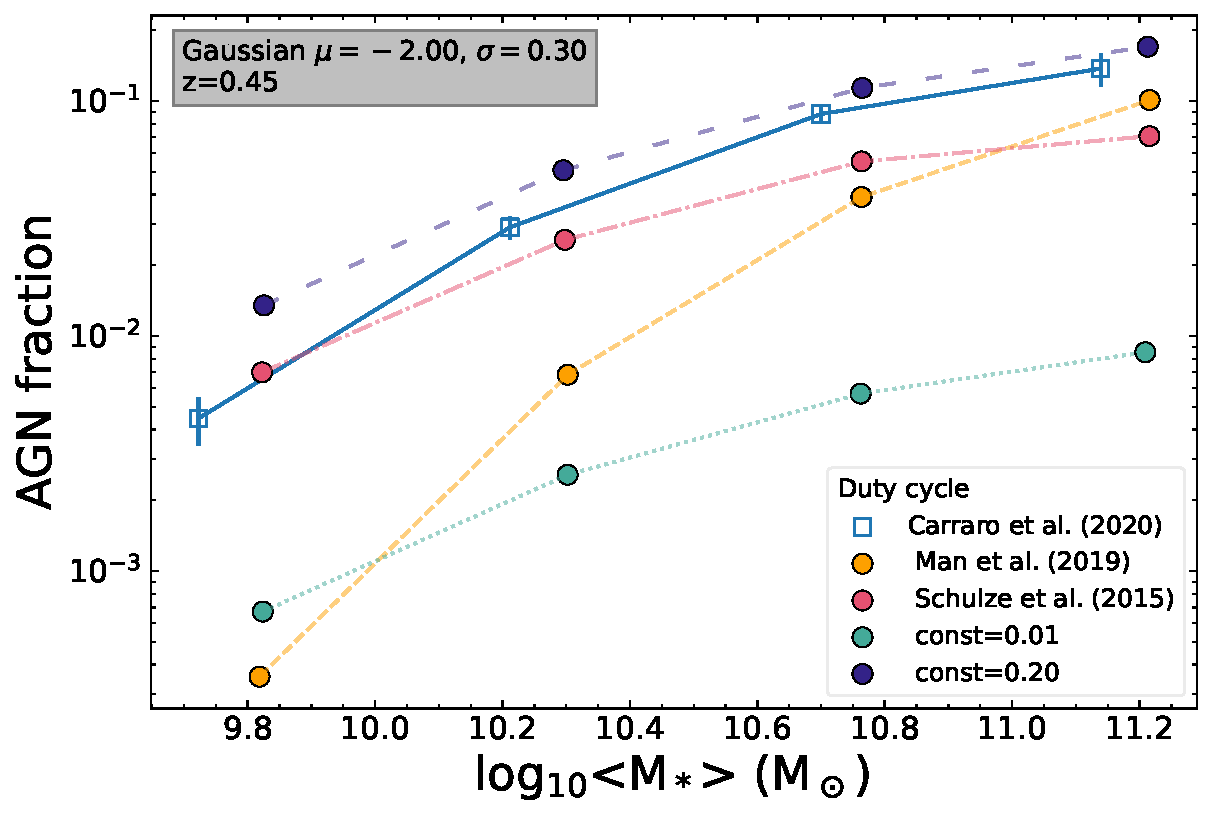
\includegraphics[width=0.49\textwidth]{Figs/Chapter3/AGN_fractions_vs_U_mean-2.00_sigma0.3_z0.45.pdf}
  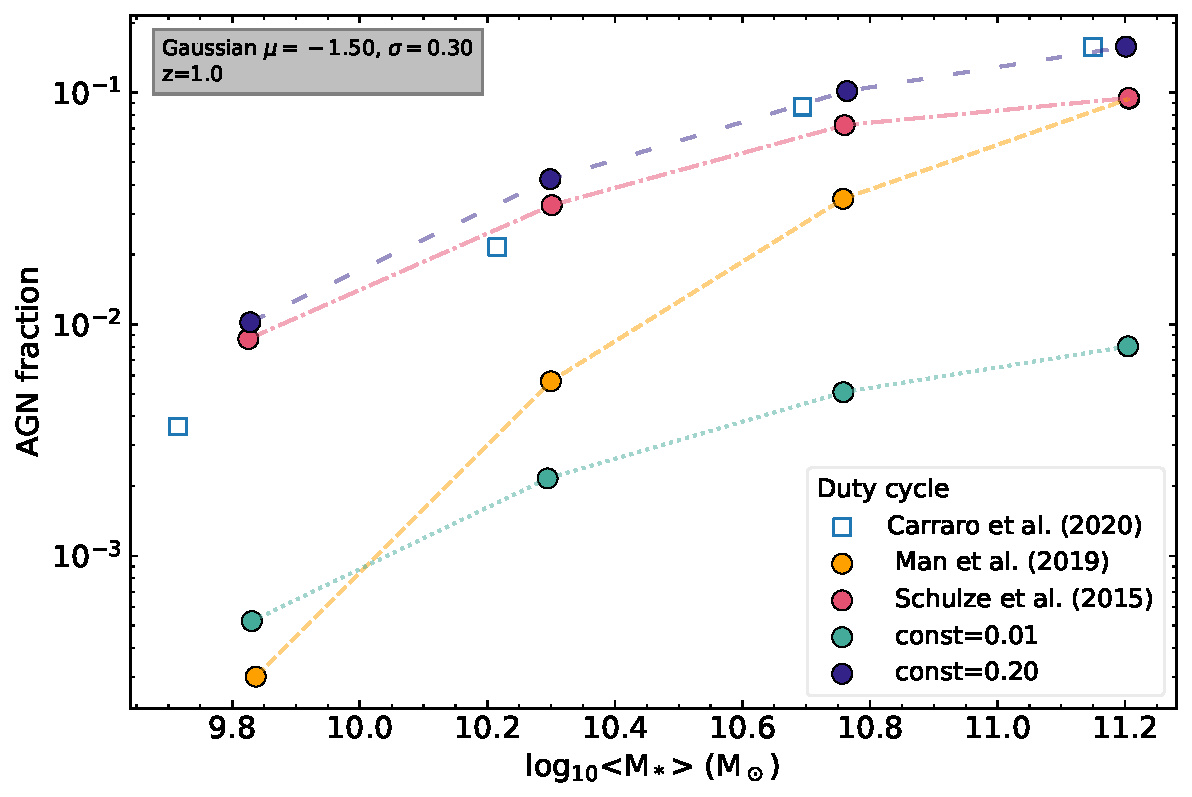
\includegraphics[width=0.49\textwidth]{Figs/Chapter3/AGN_fractions_vs_U_mean-1.50_sigma0.3_z1.0.pdf}
  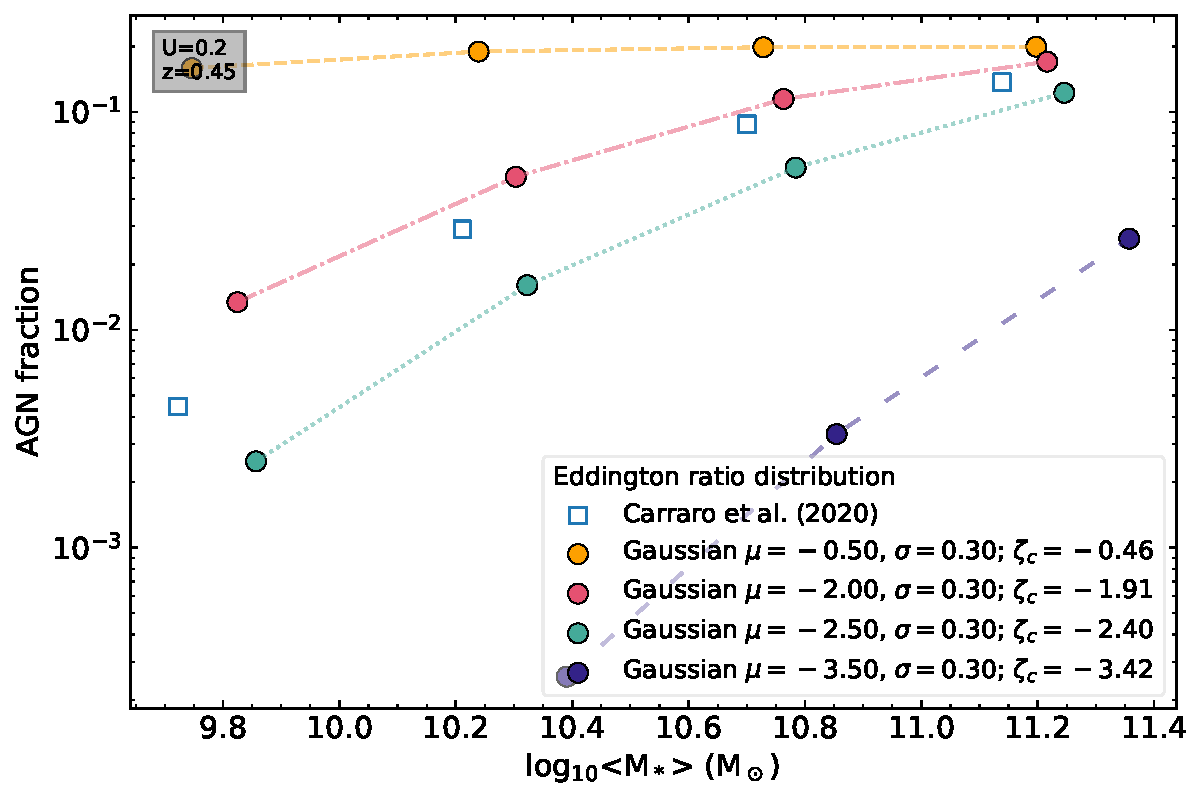
\includegraphics[width=0.49\textwidth]{Figs/Chapter3/AGN_fractions_EddRatio_U=0.2_z0.45.pdf}
  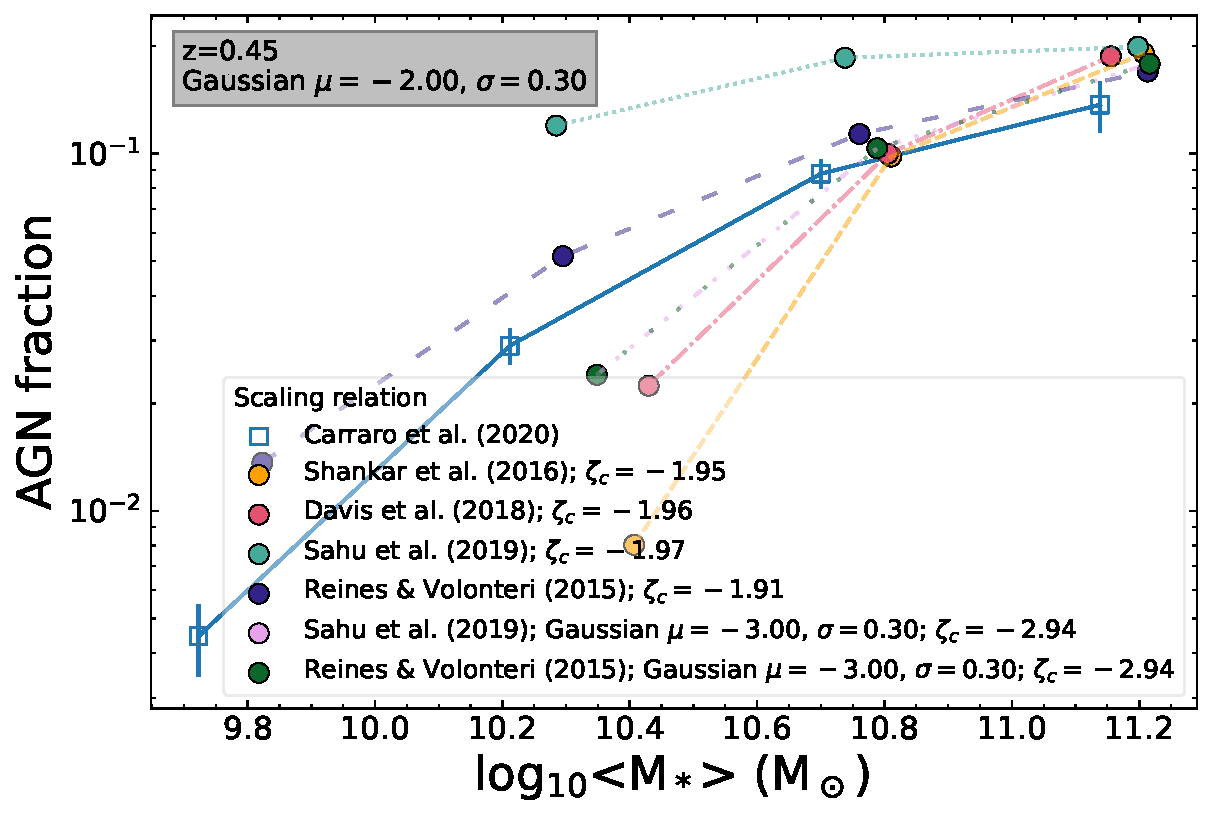
\includegraphics[width=0.49\textwidth]{Figs/Chapter3/AGN_fractions_ScalRel_comparison_z0.45.pdf}
  \caption{Dependence of the fraction of X-ray detected galaxies (AGN fraction) on the input model duty cycle (top panels),
  Eddington ratio distribution (bottom-left panel) and scaling relation (bottom-right panel)}
    \label{fig:AGN_fractions}
\end{center}
\end{figure*}
\begin{figure*}
%%%%%\vspace{8cm}
\begin{center}
  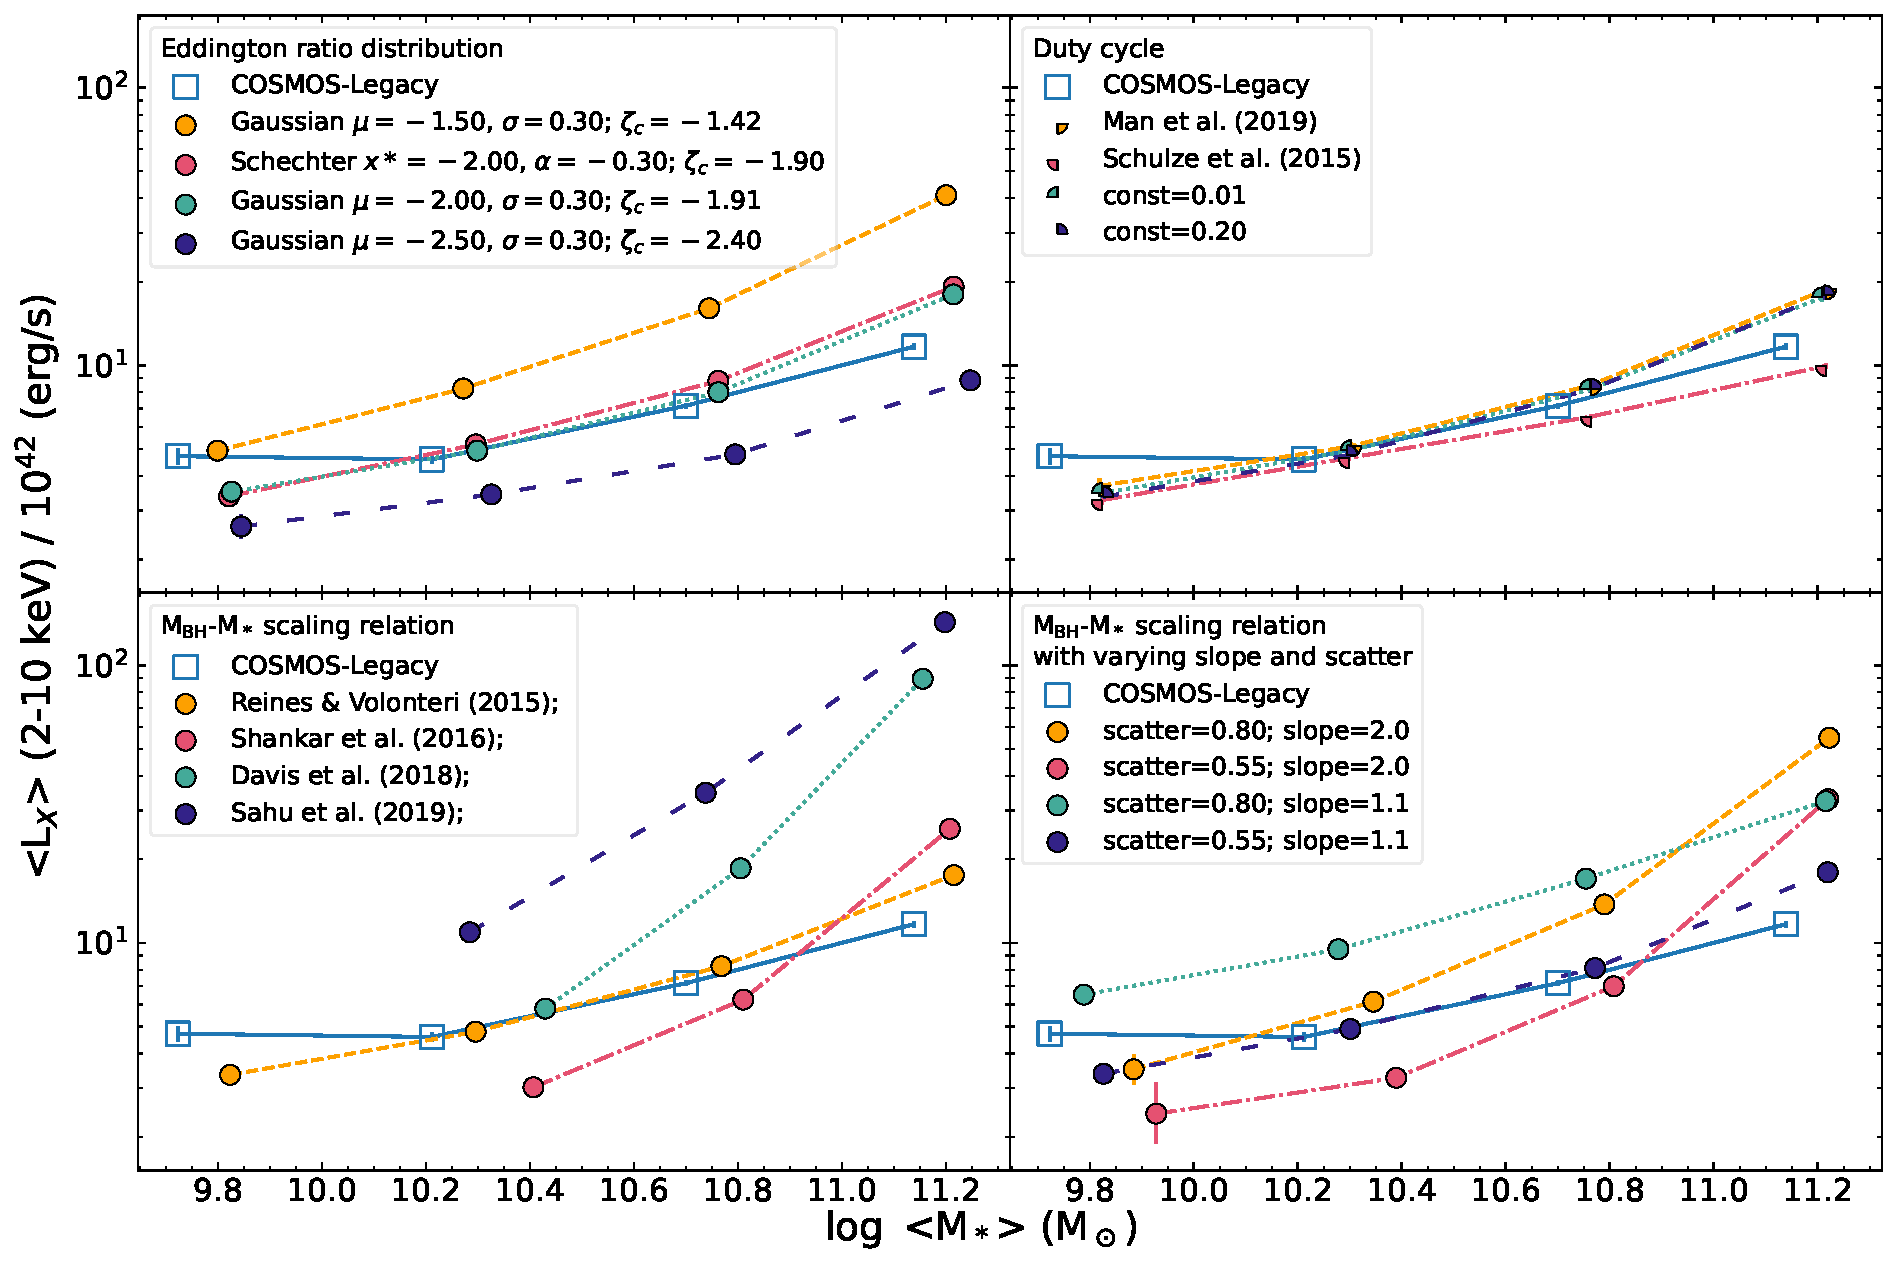
\includegraphics[width=\textwidth]{Figs/Chapter3/fig2_active_z0.45_Uconst02.pdf}
  \caption{A gallery of detected L$_{\rm X}-{\rm M}_*$ relations of detected sources at
  $z=0.45$ for star forming galaxies obtained by varying one of the input relations at a time.
  The relation that varies in each subplot is reported in the legend. 
  %Broken lines are added to the plot to guide the reader. All data-points are at $z=1$.
  Results from COSMOS X-ray detected sources at the same redshift from
  Chapter~\ref{ch:observations} are included in all plots for comparison (blue squares).
  %All data-points are at $z=1$.
  Top left: L$_{\rm X}-{\rm M}_*$ relation obtained by changing the Eddington ratio distribution function. We use a Schechter function and Gaussian function in $\log(\lambda)$ with varying mean $\mu$ and standard deviation $\sigma$ values.
  Top right: L$_{\rm X}-{\rm M}_*$ relation obtained by changing the duty cycle method.
  Bottom left: L$_{\rm X}-{\rm M}_*$ relation obtained by changing the M$_{\rm BH}-{\rm M}_*$ scaling relation. Each scaling relation is shown within its original stellar mass range of derivation.
  Bottom right: L$_{\rm X}-{\rm M}_*$ relation obtained with a toy M$_{\rm BH}-{\rm M}_*$ scaling relation where we change the logarithmic slope $\beta$ of the relation $\log {\rm M}_{\rm BH} = \alpha + \beta \log {\rm M}_*$ and increase its scatter. Original \citet{2015ApJ...813...82R} values are: $\beta=1.1$ and 0.55 dex scatter.
  }
    \label{fig:LX_M}
\end{center}
\end{figure*}
\subsection{Reproducing the measured fraction of detected galaxies} \label{ssec:Fig1}

Before showing the results on the predicted mean X-ray luminosity of detected galaxies,
we discuss if and when our model is able to match the fraction of X-ray sources directly
observed in COSMOS-Legacy as a function of stellar mass. The open blue squares in
Figure~\ref{fig:AGN_fractions} are the COSMOS-Legacy data, taken from Tables~\ref{tab:SF_prop}.
to which we associate a binomial error on the number of detected AGN and a Poisson error
on the total number of sources, combined together with standard error propagation applied to
$\frac{N_{\rm det}}{N_{\rm tot}}$.

We then compare the data with our models filtered by the flux limit of the observations, which is equal to ${\rm L}_{X,min}=10^{42}erg/s$ and ${\rm L}_{X,min}=6\times10^{42}erg/s$ at $z=0.45$ and $z=1.0$, respectively. We adopt as our reference model one characterized by a constant input duty cycle of $U=0.2$, a Gaussian Eddington ratio distribution in $\log\lambda$ peaked at $\mu=-2$, and the \MBHMS{} scaling relation from \cite{2015ApJ...813...82R}. We will show below that this choice of input parameters provides a good match to both the mean AGN X-ray luminosity and AGN luminosity function. We then vary several of the input parameters, starting from the duty cycle at both $z=0.45$ and $z=1$ (left and right top panels, respectively), the peak of the Gaussian \PLz (bottom, left panel), and the input \MBHMS{} scaling relation (bottom, right panel). It is first of all interesting to note from the top panels that, once the Gaussian $P(\log \lambda,z)$ and \MBHMS scaling relation are fixed to our reference choices, the data are consistent with an input duty cycle $U\sim0.2$ constant in both stellar/black hole mass and redshift, at least up to $z\lesssim 1$ (dark blue dashed lines in both top panels). The apparent strong increase of the AGN fraction with stellar mass is simply induced by the imposed flux limit. A too strong mass dependence in the input duty cycle, as suggested by the local fraction of optical AGN measured by \citet{2019MNRAS.488...89M} in SDSS, would be inconsistent with the data (dashed, orange lines), as well as an overall too low initial fraction (dotted, turquoise lines with $U=0.01$). 

The bottom left panel of Figure~\ref{fig:AGN_fractions} shows that a varying input \PLz{} distribution, and thus a varying characteristic $\zeta_c$, as labeled, generates widely different AGN fractions. More specifically, the higher the $\zeta_c$ the more luminous are, on average, the mock AGN, which in turn implies that proportionally less sources are removed by the cut imposed by the flux limit. We find that when $\zeta_c \gtrsim -0.5$, the observed AGN fraction is nearly identical to the input $U\sim 0.2$ (dashed, yellow line), while it rapidly diverges from the input $U\sim 0.2$ dropping towards lower mass, less luminous AGN when $\zeta_c \lesssim -2$. The right lower panel of Figure~\ref{fig:AGN_fractions} also shows that a flatter or steeper \MBHMS\ input scaling relation, such as the ones from dynamically measured $M_{\rm BH}$ by \citet[][dotted, turquoise line]{2019ApJ...876..155S} in early type galaxies and \citet[][dot-dashed, magenta line]{2018ApJ...869..113D} in late type galaxies, naturally induce a proportionally flatter or steeper AGN fraction, because they map galaxies of same stellar mass to more massive/more luminous or less massive/less luminous AGN. In conclusion, the observed AGN fraction can contribute to efficiently break the degeneracies in the input parameters (see also Section~\ref{sec:disc}), and, when combined with other independent constraints on, e.g., the BH-galaxy scaling relations and/or the Eddington ratio distributions, it is a powerful diagnostic of the intrinsic AGN duty cycle $U(y,z)$, and it can thus be used to constrain the accretion history of supermassive black holes.


\subsection{The effect of the model's inputs on the \LXMS{} relation} \label{ssec:Fig2}

In Figure~\ref{fig:LX_M} we compare the mean X-ray luminosity of detected active galaxies in a given bin of stellar mass, which in what follows we will continue labeling simply as \LX{} (Eq.~\ref{eq:meanLx}), with several different model predictions. To pin down the input parameters that mostly control the \LXMS\ relation, we explore in Figure~\ref{fig:LX_M} how the relation varies by changing, from top left to bottom right, the \PLz\ , the duty cycle, the full \MBHMS\ relation, and only the slope/scatter of the \citet{2015ApJ...813...82R} relation, as labeled. All the mocks are generated at $z=0.45$, though the results are applicable to all redshifts, as further discussed below. In Figure~\ref{fig:LX_M} the data refer to only the subsample of star forming, main sequence galaxies. As anticipated in Sec~\ref{sec:model} and Eq.~\ref{eq:meanLx}, the mean \LX\ should in principle be weighted by the fractional number of detected sources within a given star formation class (e.g., quiescent, star forming, starbursts). However, this additional weighting can be neglected as it is canceled out in Eq.~\ref{eq:meanLx}, being a constant in each bin of stellar mass.

\begin{figure*}
%%%%%\vspace{8cm}
\begin{center}
  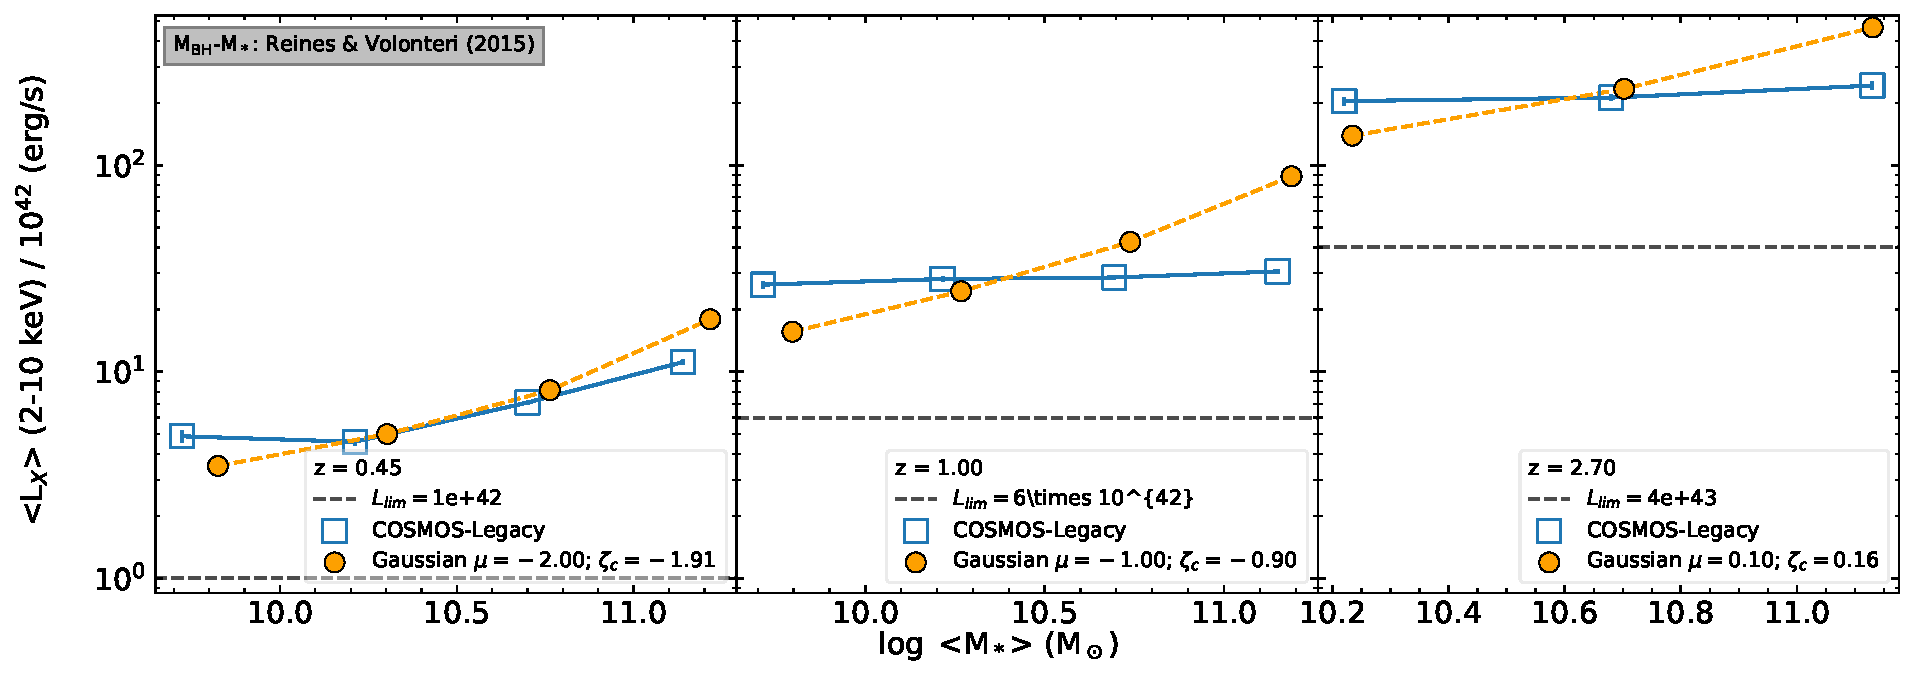
\includegraphics[width=\textwidth]{Figs/Chapter3/fig3_active.pdf}
  \caption{The L$_{\rm X}-{\rm M}_*$ relations at $z=0.45$ (left panels), $z=1.0$
  (central panels) and $z=2.7$ (right panels) obtained by assuming a M$_{\rm BH}-{\rm M}_*$
  scaling relation from \citet{2015ApJ...813...82R} and a Gaussian in $\log (\lambda)$ with
  standard deviation $\sigma=0.3$~dex. We vary the Eddington ratio distribution in order to
  reproduce the observational results from the COSMOS-Legacy detected sources selected in Chapter~\ref{ch:observations}.
  Black dashed lines represent the survey luminosity limits.}

    \label{fig:LX_M_redshift}
\end{center}
\end{figure*}


\subsection{Reproducing the \LXMS\ relation through cosmic time}

In this Section we extend the comparison to data on the \LXMS\ relation at different redshifts. We showed in the previous Section that the \LX\ can provide valuable constraints on the mean Eddington ratio of active BHs. Thus, by studying the \LXMS\ at different redshifts and galaxy stellar masses, we can build a more comprehensive view of how BHs accrete at different epochs and in different host galaxies.
The data point to a steady decrease of the mean \LXMS\ luminosity with cosmic time at fixed host galaxy stellar mass. As discussed above, this decreasing trend could be interpreted either as a progressive decline in the normalization of the \MBHMS\ relation and/or in the characteristic $\zeta_c$. The latest data suggest a rather weak evolution in the \MBHMS\ relation up to at least $z\sim 2.5$ \citep[e.g.,][]{2020ApJ...889...32S,2020MNRAS.493.1500S} thus favoring, in our approach, a steady decrease in $\zeta_c$, which would also be in line with independent observations \citep[]{Kollmeier06} and continuity equation models \citep[][]{Shankar13Acc,Aversa15}.


The top panels of Figure~\ref{fig:LX_M} clearly show that while the normalization of the \LXMS\ relation is strongly controlled by the characteristic Eddington ratio $\zeta_c$ (left panel), it has a negligible dependence on the input AGN duty cycle (right panel). This behavior is expected as the \LX\ in Eq.~\ref{eq:meanLx} is an average luminosity calculated only on the fraction of active sources, and as such it is largely independent of the number of BHs active in a given bin of stellar mass, but strongly dependent on the {\emph{rate}} at which these BHs are accreting. We show in the top left panel of Figure~\ref{fig:LX_M} that a Schechter or Gaussian \PLz\ yield the same mean X-ray luminosity \LX\ at fixed stellar mass as long as their $\zeta_c$ are the same (dotted turquoise and dot-dashed magenta lines). It is indeed the characteristic Eddington ratio $\zeta_c$, and not the overall shape of the \PLz\ input distribution, to determine the level of mean X-ray luminosity in active galaxies at fixed stellar mass and
fixed \MBHMS\ relation. Nevertheless, some constraints even on the shape of the \PLz\ could be derived from our methodology. For example, assuming a steeper/flatter faint end in the input Schechter \PLz\ function, would induce a lower/higher $\zeta_c$. To then preserve the same $\zeta_c$ necessary to match the observed \LXMS\ relation, would in turn require a shift in the knee of the Schechter function, and the new combination of faint end slope and knee can then be tested against the AGN luminosity function (which we further discuss below). It is relevant to reiterate at this point that the observations are only sensitive to Eddington ratios corresponding to luminosities above the survey flux limit (Eq.~\ref{eq:zeta_c}), and thus are sensitive only to portion of the \PLz\ above the minimum Eddington ratio detectable in the sample.

Some residual, weak dependence on the duty cycle may be visible in the right panel of Figure~\ref{fig:LX_M} especially towards higher stellar masses (dote-dashed, magenta line). This (tiny) dependence of the \LXMS\ relation on the input duty cycle is a simple byproduct of the scatter in the \MBHMS\ relation and of our definition of input duty cycle: \UMBHz\ is dependent on BH mass, and thus at fixed stellar mass, a variety of BHs with different weights could contribute to the mean \LX\, slightly altering its final value depending on the shape (not the normalization) of the input duty cycle \UMBHz{}.

The bottom left panel of Figure~\ref{fig:LX_M} shows instead a close link between the normalization of the input \MBHMS\ relation and the normalization in the \LXMS\ relation: at fixed $\zeta_c$, a lower \MBHMS\ relation will result in a proportionally lower \LXMS\ relation, and vice versa. This causal link between the two relations naturally arises from the proportionality between X-ray luminosity and BH mass, which in turn is linked to the host galaxy stellar mass via the \MBHMS\ relation. The right panel of Figure~\ref{fig:LX_M} shows the variations in the \LXMS\ relation for the same input \MBHMS\ relation with varying slope or scatter, as labeled. A steeper/shallower \MBHMS\ scaling relation will result in a proportionally steeper/shallower \LXMS\ relation, while a lower/higher scatter will decrease/increase the normalization of the \LXMS\ relation, mainly due to the lower/larger contribution of active BHs, especially the more massive and luminous ones. It is thus clear from Figure~\ref{fig:LX_M} that the slope and normalization of the input \MBHMS\ relation, as well as the input $\zeta_c$, all play a significant, and in fact degenerate, role in shaping the \LXMS\ relation. For example, a flatter slope in the \MBHMS\ relation or a mass-dependent $\zeta_c$, progressively decreasing at larger masses, could both produce a flatter slope in the \LXMS\ relation. Also, decreasing $\zeta_c$ with increasing BH mass could indeed reconcile the our observational results from Chapter~\ref{ch:observations} with a steeper \MBHMS\ relation as calibrated in the local Universe \citep[e.g.,][]{2016MNRAS.460.3119S,2018ApJ...869..113D}. If the scaling relation between BHs and their hosts is constrained via independent methods, such as AGN clustering \citep[e.g.,][]{ShankarNat,Allevato21}, then the \LXMS\ relation can be used to constrain the mean $\zeta_c$ as a function of galaxy stellar mass and redshift, as further discussed below.

\begin{figure*}
	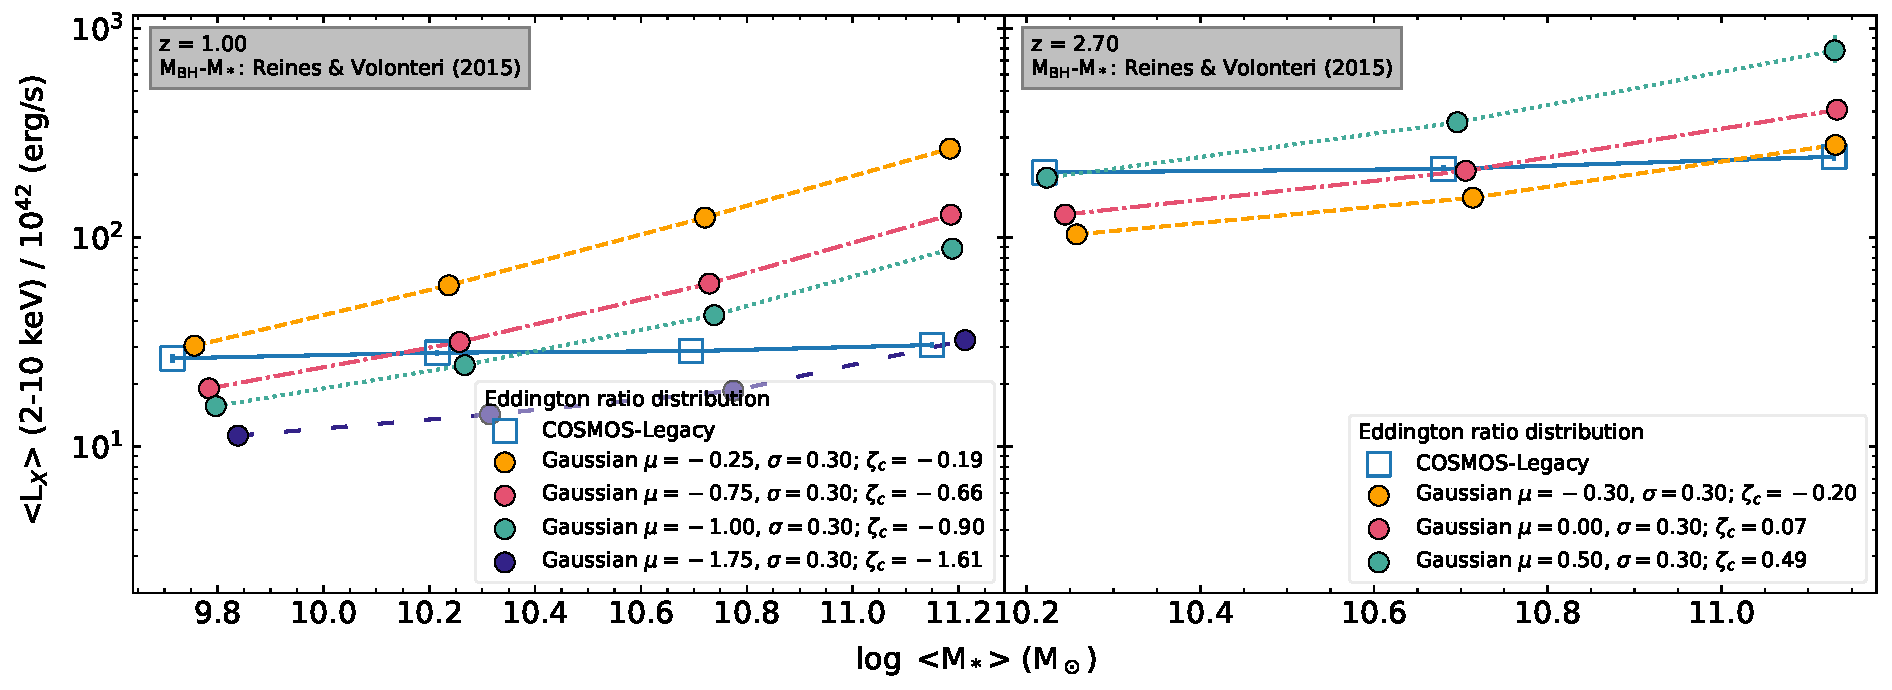
\includegraphics[width=\textwidth]{Figs/Chapter3/Best_Edd_for_mass_active_z2.7.pdf}
	\caption{$L_X-M_*$ relation for active galaxies at $z=1.0,2.7$, looking for a $\zeta_c$ that fits each M$_*$ bin.}
	\label{fig:LX_foreach_M}
\end{figure*}

In Figure~\ref{fig:LX_M_redshift} we show the predicted \LXMS\ relation for mock catalogs at $z=0.45,1.0,2.7$ (left, central and right panels respectively), generated by assuming as a reference the \citet{2015ApJ...813...82R} \MBHMS\ relation. 
At each redshift we plot the models with an input \PLz\ Gaussian distribution with a $\mu$ value (the corresponding $\zeta_c$ values are very similar being Gaussian distributions) chosen in a way to match the central value of the \LXMS\ distribution at each redshift.
We find that, as can be better seen in Fig.\ref{fig:LX_foreach_M}, assuming a strictly constant \MBHMS\ relation, to reproduce the data we would need a drop of a factor of $\gtrsim 100$ in the characteristic Eddington ratio $\zeta_c$ from $z\sim 2.7$ to $z\sim 0.45$, which mirrors the fast drop in mean Eddington ratio also derived in some observational data and continuity equation results \citep[see, e.g., Fig. 12 in][]{Shankar13Acc}. We also note that at $z \gtrsim 1$, on the assumption that the input \MBHMS\ relation remains constant in both slope and normalization, the models tend to produce a \LXMS\ relation steeper than what observed, which in turn would require a $\zeta_c$ decreasing with increasing stellar mass by a factor $\lesssim 3$ to improve the match to the data. A systematically lower mean Eddington ratio for more massive galaxies would imply that their more massive BHs should have grown faster, the so-called {\emph downsizing} trend, already introduced and discussed in the previous Chapters, in which more massive galaxies/BHs form faster than less massive galaxies/BHs. The results in Figure~\ref{fig:LX_M_redshift} taken at face value suggest that BHs would be accreting close to their Eddington limit at $z\gtrsim 2.5$, and then rapidly shut off at lower redshifts, especially for more massive galaxies. Indeed, continuity equation models clearly show that more massive BHs have formed most of their mass by $z\sim 1$ \citep[e.g.,][]{2004MNRAS.351..169M,2020MNRAS.493.1500S}.



\begin{figure*}
\begin{center}
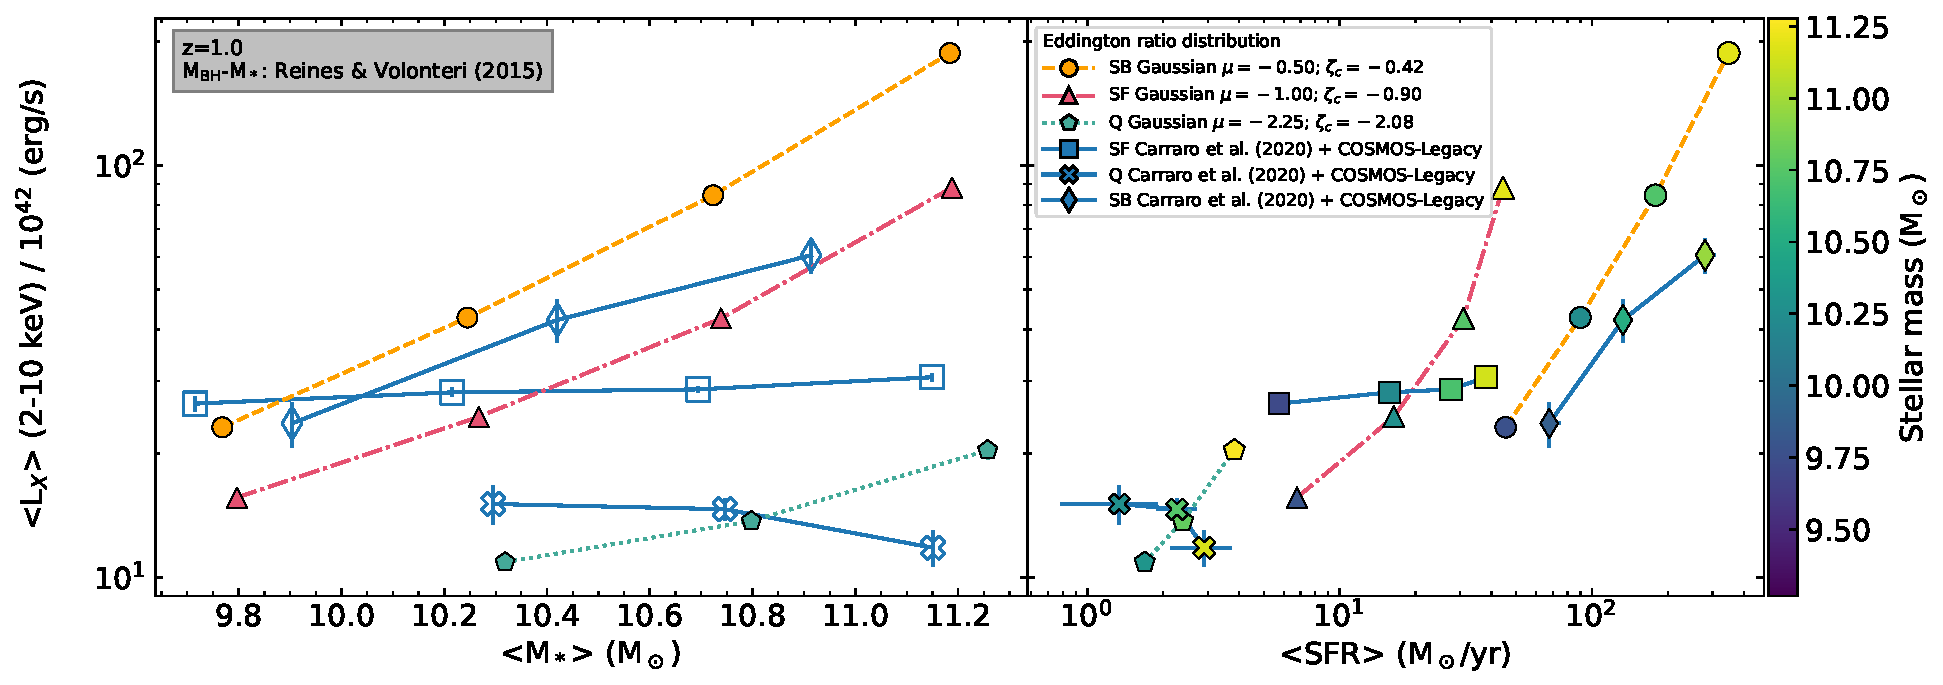
\includegraphics[width=\textwidth]{Figs/Chapter3/fig4_1.0_active.pdf} 
  \caption{L$_{\rm X}$ as a function of ${\rm M}_*$ (left) and SFR (right). L$_{\rm X}$ are
  obtained at %$z=0.45$ and
  $z=1.0$ for detected galaxies with a \citet{2015ApJ...813...82R} M$_{\rm BH}-{\rm M}_*$
  scaling relation and with a Gaussian Eddington ratio distribution as shown in the legend,
  with a $\sigma=0.3 dex$. In the right panel, SFRs are obtained using the fits from
  \ref{table:all_fitpar} for star-forming (SF), quiescent (Q) and starburst (SB) galaxies,
  and data points are color coded according to ${\rm M}_*$. All relations are compared with
  results from COSMOS data from Chapter~\ref{ch:observations}}
    \label{fig:SFQSB_active}
\end{center}
\end{figure*}

\subsection{Reproducing the \LXMS\ relation in starburst, main-sequence and quiescent galaxies} \label{subsec:SFQSB}

So far we have mostly focused on comparing model predictions with the mean \LXMS\ relation
of star forming main sequence galaxies, which are the vast majority of the detected  active galaxies in COSMOS-Legacy. However, AGN activity is routinely detected also in other galaxy life phases. In Figure~\ref{fig:L_X} we showed that, at least at $z<2.25$, starbursts, star forming and quiescent galaxies are characterized by distinct \LXMS\ relations, which are similar in slope but differ in normalization by a factor of $\sim 10$ when moving from quiescent galaxies, with the lowest average \LX, to the starbursts, with the highest average \LX\ at fixed stellar mass. In the context of our approach, this offset in \LX\ at fixed stellar mass could be explained either by a systematic difference in the characteristic Eddington ratio $\zeta_c$ and/or by a systematic offset in the normalization of the \MBHMS\ relation, when moving from quiescent to starforming galaxies. In this Section we proceed with a systematic comparison of our models with the COSMOS-Legacy data focusing on the dependence of the \LXMS\ relation on galaxy type at fixed redshift, specifically at $z=1$, though the conclusions we will retrieve below are quite general and can be easily extended to other redshift bins.
 
In the left panel of Figure~\ref{fig:SFQSB_active} we explore mocks with a constant input
\MBHMS\ relation from \citet{2015ApJ...813...82R}, but characterized by distinct $\zeta_c$, as labeled (circles, triangles, and pentagons), against the \LXMS\ relation measured for the three types of galaxies studied in Chapter~\ref{ch:observations} (blue diamonds, squares and crosses for starbursts, star forming, and quiescent galaxies, respectively). Reproducing the steep increase in mean \LX\ at fixed ${\rm M}_*$ requires, as expected, a proportionally higher value of $\zeta_c$ in main sequence and starburst galaxies, assuming the same \MBHMS\ relation. We stress that the calculation of the mean \LX\ of each galaxy type via Eq.~\ref{eq:meanLx} would require an additional statistical weight specifying the relative contribution of each galaxy type to the total number of detected active galaxies. As this weight is constant in each stellar mass bin, it would however cancel out when applied to the numerator and denominator of Eq.~\ref{eq:meanLx}.
In the right panel of Fig.~\ref{fig:SFQSB_active} we show the SFRs of the entire sample from Chapter~\ref{ch:observations} against the luminosity of the X-ray detected sources only. We decided not to use the SFRs from the detected sample since the tracers used for their estimation (IR and UV luminosity) may be polluted by AGN emission and the IR stacking may not achieve a significant signal-to-noise with the low number statistics from this subsample, both leading to non-representative SFRs for these galaxies.

Interestingly, it is apparent from Figure~\ref{fig:SFQSB_active} that the observed \LXMS\
relation in starburst galaxies is not a simple power law but tends to show a break
that becomes more pronounced in more massive galaxies of mass
$\log (M_*/M_{\odot}) \gtrsim 10.5$ and at lower redshifts. In our modeling,
this feature could be naturally reproduced with a further decrease in $\zeta_c$ in the
most massive galaxies in our sample, which would align with the idea of downsizing, as
discussed above. This result supports the view that, already in the early starburst phase,
more massive galaxies and their central BHs have accreted their mass earlier and are
now in their declining phase, as predicted by some models \citep[e.g.,][]{2018ApJ...857...22L}. We stress
that the downsizing in $\zeta_c$ would be even more pronounced if steeper \MBHMS\ relations
were adopted in input. The right panel of Figure~\ref{fig:SFQSB_active} shows that our
chosen values of $\zeta_c$ that match the \LXMS\ relation for each galaxy type also
reproduce, at the same time, their respective ${\rm L}_{\rm X}-{\rm SFR}$ relations, where
the SFR is assigned to each galaxy type based on their observed underlying
${\rm SFR}-{\rm M}_*$ relation. 

An alternative way to explain the different normalizations of starburst and quiescent galaxies
in the \LXMS\ plane would be to adopt the same $\zeta_c$ for all galaxy types and progressively
increase the normalization of the \MBHMS\ scaling relation when moving from quiescent to
starburst galaxies.
We however disfavor such a model. Direct measurements of the \MBHMS\ scaling relation in
AGN within a variety of host galaxies
\citep[e.g.,][and references therein]{2015ApJ...813...82R,2019MNRAS.485.1278S,2020ApJ...889...32S},
have all revealed normalizations that are lower than those typically measured locally
in dynamically measured BHs, possibly due to some biases in the latter
\citep[e.g.,][]{2016MNRAS.460.3119S}. In particular, BHs in local elliptical, quiescent
galaxies seem to be the most massive ones at fixed host galaxy stellar mass among all
samples of local active and normal galaxies (see, for example, Figure 8 in
\citealt{2015ApJ...813...82R}). In addition, also the analysis of the clustering of active,
mostly starforming, galaxies at fixed BH mass favors \MBHMS\ scaling relations with a
normalization lower than the one measured for local quiescent, early-type galaxies
\citep[e.g.,][]{ShankarNat,Allevato21,Viita21}. Direct (or indirect) comprehensive
measurements of the \MBHMS\ scaling relation in active starburst galaxies are still
unavailable. However, theoretical models suggest that the ratio between BH mass and host
galaxy stellar mass in the starburst phase should, if anything, be lower than what observed
locally, as the BH grows from a relatively small seed within a host forming stars at
exceptionally high rates \citep[see, e.g.,][their Figure 3]{2014ApJ...782...69L}. More generally, these
models suggest that, from an evolutionary point of view, quiescent galaxies should be older
galaxies with larger BHs at fixed stellar mass
\citep[e.g.,][]{Ciras05,Granato06,2006ApJ...650...42L,shankar06,2018ApJ...857...22L}.

All in all, the evolutionary picture that could be extracted from
Figure~\ref{fig:SFQSB_active} is one in which the central BH and its host galaxy move around
a similar \MBHMS\ scaling relation throughout their lifetime. They could start from a
main-sequence or even starburst, gas-rich phase, evolving at an almost constant (specific)
SFR, as also proposed by theoretical models \citep[e.g.][]{2014ApJ...782...69L, Aversa15} and direct
observations (Chapter~\ref{ch:observations}, and then gradually switch off their accretion
and star formation due to internal gas consumption, thus gradually reducing their SFR and
accretion onto the central BH (right panel of Figure~\ref{fig:SFQSB_active}). 

\begin{figure*}
	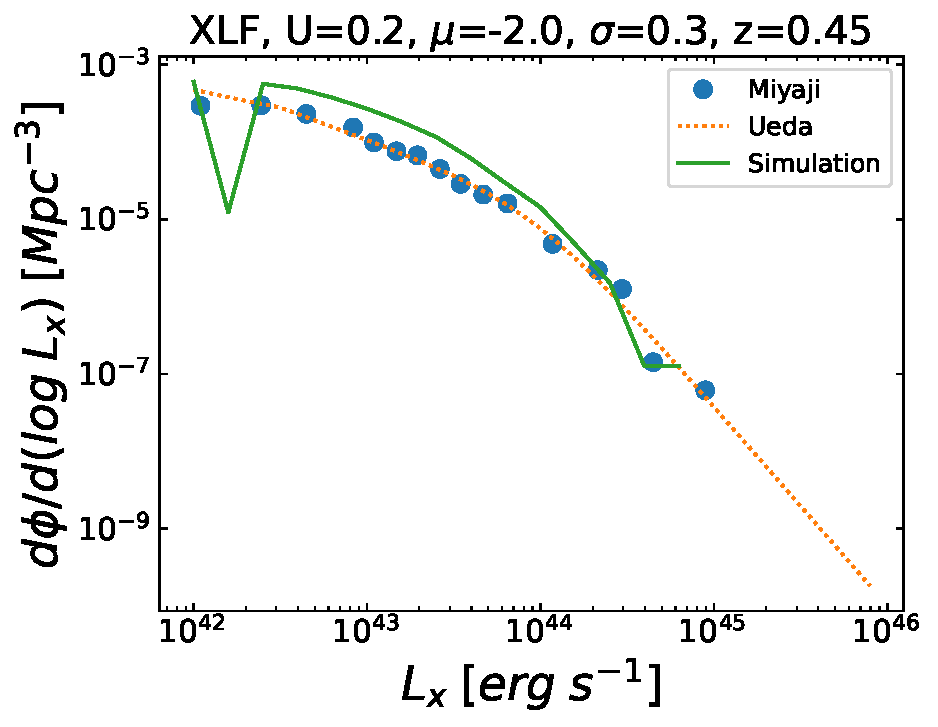
\includegraphics[width=0.49\textwidth]{Figs/Chapter3/XLF_z0.45_mean-2.00_sigma0.30_const0.2.pdf}
	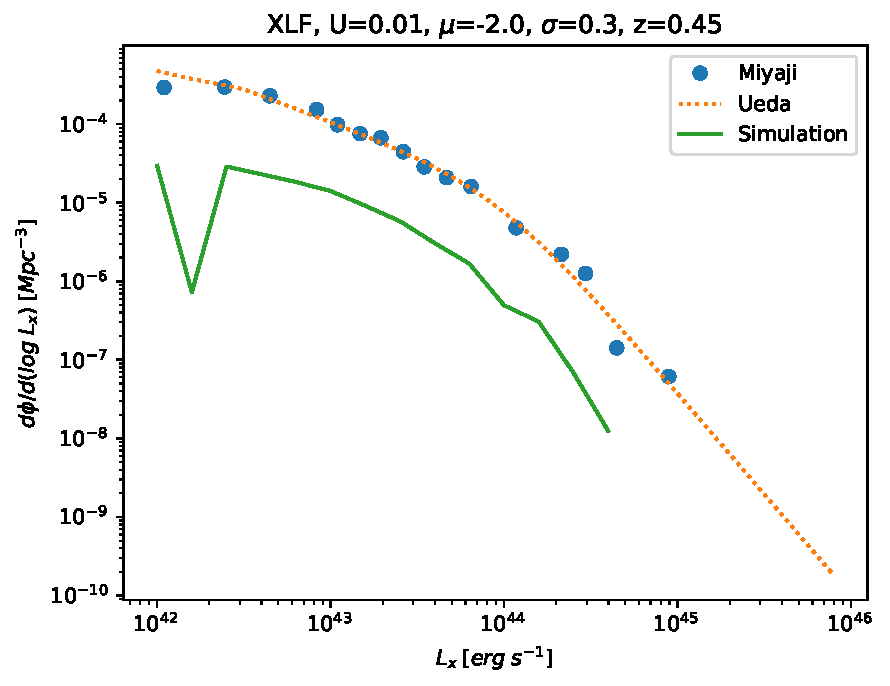
\includegraphics[width=0.49\textwidth]{Figs/Chapter3/XLF_z0.45_mean-2.00_sigma0.30_const0.01.pdf}
	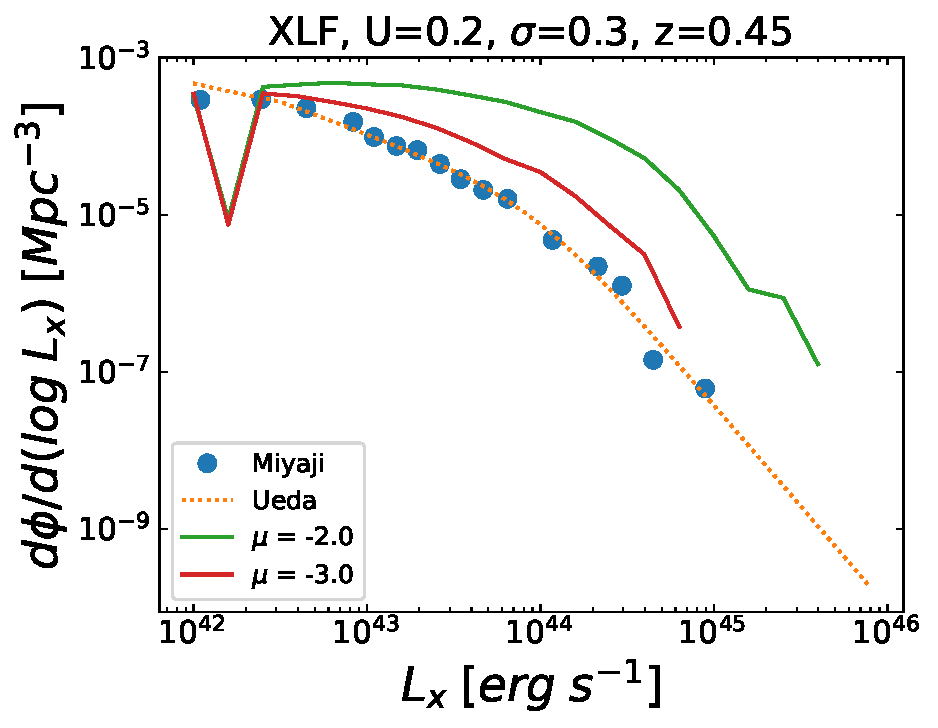
\includegraphics[width=0.49\textwidth]{Figs/Chapter3/XLF_z0.45_sigma0.3mean_Sahu19_const0.2.pdf}
	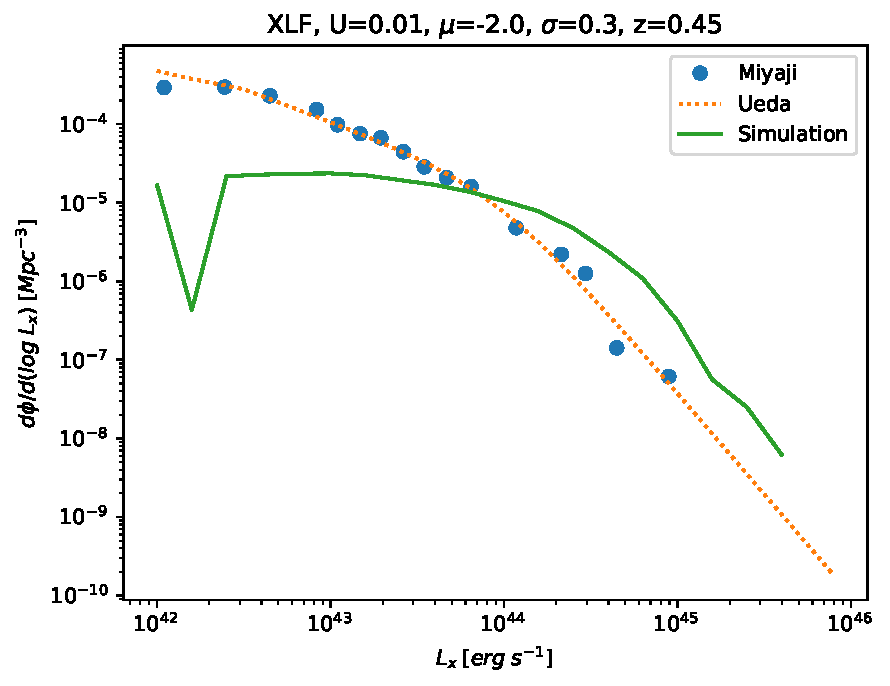
\includegraphics[width=0.49\textwidth]{Figs/Chapter3/XLF_z0.45_mean-2.00_sigma0.30Sahu19_const0.01.pdf}
	\caption{XLF from the models using the Eddington ratio better representing the $L_X$ of the data at $z=0.45$. Top panels: Using \citet{2015ApJ...813...82R} scaling relation, varying the duty cycle U=0.2 (left) and U=0.01 (right). Bottom panels: Using \citet{2019ApJ...876..155S} scaling relation, varying the duty cycle U=0.2 (left) and U=0.01 (right). Models are compared with data from \citet{2014ApJ...786..104U} and \citet{2015ApJ...804..104M} at the same redshift.}
	\label{fig:XLF}
\end{figure*}

\section{Discussion}\label{sec:disc}

We showed in the previous Sections that the mean \LXMS\ relation of X-ray detected active
galaxies is a powerful tool to constrain the mean accretion rate of active BHs $\zeta_c$ as
a function of time and BH mass, and in ways largely independent of the duty cycle. When
coupled to other independent probes, the \LXMS\ can thus provide an invaluable support in
breaking the degeneracies in the accretion parameters of supermassive BHs. 
For example, as discussed in Section 2, the AGN X-ray luminosity function is a convolution
of the underlying BH mass function, which mostly depends on the BH-galaxy scaling relations
\citep[e.g.,][]{Salucci99}, the intrinsic fraction of active BHs as a function of BH
mass (the duty cycle $U(y,z)$), and the normalized Eddington ratio distribution \PLz\
\citep[see, e.g.,][and references therein]{Shankar13Acc}. Thus, knowledge of the AGN X-ray
luminosity function and of the characteristic mean Eddington ratio $\zeta_c$ from independent
observables, could shed light on the duty cycle, once a robust estimate of the underlying
BH-galaxy scaling relation is available from, e.g., AGN clustering measurements
\citep[see discussion in][]{ShankarNat,Allevato21,Viita21}. 

Figure~\ref{fig:XLF} shows a few examples of the dependencies of the AGN luminosity function
on the most relevant model input parameters. We compare the observed X-ray AGN luminosity
function\footnote{Both luminosity functions do not include Compton-thick sources, thus our
duty cycle \UMBHz\ refers to the total fraction of Compton-thin AGN, i.e., those with
$\log N_H<24\, {\rm cm^{-2}}$.} by \citet[][orange dotted lines]{2014ApJ...786..104U}
and \citet[][blue filled circles]{2015ApJ...804..104M}, with the predictions of our
reference model with a constant duty cycle $U=0.2$, a \MBHMS\ relation from
\citet{2015ApJ...813...82R}, and a Gaussian \PLz\ with $\mu=-2$, a combination able to
simultaneously reproduce the observed fraction of X-ray AGN (Figure~\ref{fig:AGN_fractions})
and mean \LXMS\ relation (Figure~\ref{fig:LX_M}). Despite the crudeness of our model, the
top-left panel of Figure~\ref{fig:XLF} shows that our reference mock (solid green line) is
able to broadly reproduce the data at all luminosities within a factor of $\lesssim 2$,
without any extra fine-tuning. On the other hand, when switching to a \MBHMS\ relation with
a higher normalization than the one calibrated by \citet{2015ApJ...813...82R}, such as the
one by \citet{2019ApJ...876..155S}, would tend to significantly overproduce the observed AGN
luminosity function, an effect induced by the new \MBHMS\ relation which maps galaxies to
more massive BHs and thus more luminous AGN \citep[e.g.,][]{ShankarNat}. To recover the match
to the AGN luminosity function with the new \MBHMS\ relation we would require a mean Eddington
ratio $\zeta_c$ significantly lower by more than an order of magnitude,
as shown in the bottom, left panel (solid, red line), which allows to systematically shift the predicted
luminosity function by a factor of $\gtrsim 10$ to fainter X-ray luminosities, in better
agreement with the data. Although such a low value of $\zeta_c$ could still generate a
\LXMS\ relation in broad agreement with the data, at least at larger stellar masses (by
simply proportionally lowering the violet dashed model in the bottom, left panel of
Figure~\ref{fig:LX_M}), and also with the observed AGN fraction (pink double dot-dashed
line in the bottom right panel of Figure~\ref{fig:AGN_fractions}), it would be inconsistent
with independent measurements of the mean Eddington ratios at similar redshifts
\citep[e.g.,][]{H09,Kauff09,2019MNRAS.484.4360A}. Alternatively, we could keep the reference
value of $\zeta_c$ but decrease the duty cycle to $U=0.01$, as shown in the solid lines
reported in the right panels of Figure~\ref{fig:XLF}. This solution improves the match between
the model with higher normalization in the \MBHMS\ relation and the observed AGN luminosity
function, at least at the bright end (bottom right panel). However, such a low value of the
duty cycle $U=0.01$ is inconsistent with the much higher fraction of AGN detected in
COSMOS-Legacy (Figure~\ref{fig:AGN_fractions}).

Our current work is able to provide additional clues and empirical evidence in support of
the (complex) models of supermassive BH evolution in galaxies. According to the standard
picture of the early phases of the co-evolution of galaxies and their central BHs
\citep[e.g.,][]{Granato06,Hopkins06,2018ApJ...857...22L}, galaxies undergo a first rapid, gas-rich and
strong burst of star formation, during which a (seed) BH can substantially grow at or above
the Eddington limit, followed by a more regular and then quiescent phase during which both
the star formation and the accretion onto the central BH drop substantially. We already
showed in the left panel of Figure~\ref{fig:SFQSB_active} that, in the context of our modeling,
when assuming a constant or slowly varying underlying \MBHMS scaling relation, the data tend to
favor an evolving characteristic Eddington ratio $\zeta_c$, steadily declining when the
galaxy transitions from the starburst to the quiescent phase, and we suggested, based on the
comparison with the L$_X$-SFR relation (right panel of Figure~\ref{fig:SFQSB_active}), that
this temporal trend in BH accretion rate should be closely mirrored by the star formation
in the host galaxy, in agreement with the expectations from theoretical models. Here we
further elaborate on this idea.
In the previous Chapter, see, e.g., Figure~\ref{fig:SF_BH_all}, we showed that
main-sequence and quiescent galaxies share similar ratios of BHAR and SFR at all probed
cosmic epochs, suggesting that the two processes are indeed linked together throughout
different galaxy phases.  
In fact, the mean BHAR/SFR can be written as
${\rm BHAR/SFR} \propto L_{bol}/{\rm SFR} \propto 10^{\zeta_c} {\rm M}_{\rm BH}/(k {\rm M}_*)$
, where $k={\rm SFR}/{\rm M}_*$ is the specific SFR. Thus, at fixed
${\rm M}_{\rm BH}/{\rm M}_*$, a similar BHAR/SFR ratio as the one observed in star forming
and quiescent galaxies, would be induced by a proportional decline in characteristic
Eddington ratio $\zeta_c$ and specific SFR $k$ within a bin of stellar mass. Analogously,
the significantly lower BHAR/SFR in starbursts with respect to quiescent/star forming galaxies,
as shown in Fig.~\ref{fig:SF_BH_all}, would be naturally interpreted as a
proportionally higher specific SFR $k$ 
and roughly constant or slightly higher $\zeta_c$ in these young gas rich systems, as
predicted by some BH evolutionary models \citep[e.g.,][]{2014ApJ...782...69L,Aversa15}.

\section{Conclusions}\label{sec:concl}

In this work we use statistical semi-empirical models to generate accurate mock catalogs of active galaxies, which we analyze in the same manner as in the comparison observational sample from Chapter~\ref{ch:observations}. Our goal is to unveil the input parameters driving the \LXMS\ relation. We start from a halo mass function at a given redshift, we assign galaxies and BHs to dark matter haloes via the most up-to-date empirical stellar-halo and \MBHMS\ relations, and we assume a SFR depending only on stellar mass and redshift. We explore a range of Eddington ratio distributions \PLz, \MBHMS\ scaling relations and duty cycles \UMBHz. Our results can be summarized as follows:
 \begin{itemize}
    \item In agreement with previous findings \citep[see, e.g.,][]{2012ApJ...746...90A,Shankar13Acc}, the apparent increase of AGN detections towards high stellar masses, i.e., the ``observed'' AGN fraction, is not necessarily caused by AGN being more frequent in more massive galaxies, but we find that it is mostly a consequence of the X-ray survey flux limit, which prevents the detection of the faintest sources with a higher probability of being located in lower mass galaxies.
    \item The mean \LXMS\ (or L$_{\rm X}$-SFR) relation in detected BHs is largely independent
    of the AGN duty cycle, but strongly depends on the shape, normalization and scatter of
    the underlying \MBHMS\ scaling relation and on the characteristic Eddington ratio
    $\zeta_c$, which play a degenerate role in linking the mean \LX\ with the BH mass. 
    \item When assuming a roughly constant \MBHMS\ relation with time, as indicated by many
    recent observations, current X-ray data on the \LXMS\ relation favor models with a mean
    Eddington ratio of a few percent at $z=0.45$ and rapidly approaching the Eddington limit
    at $z\sim 3$, in broad agreement with a variety of independent data sets and theoretical
    models. 
    \item At fixed redshift $z \gtrsim 1$, the same data sets also show evidence for downsizing, with the most massive BHs having accreted their mass more rapidly than less massive BHs.  
    \item At fixed redshift, the \LXMS\ relation increases by nearly an order of magnitude
    in normalization when moving from quiescent to starburst galaxies. Our models suggest
    that, on the reasonable assumption of a constant \MBHMS\ relation, this increase in mean
    \LX\ is mostly induced by the mean $\zeta_c$ being much higher during the starburst,
    gas-rich phase, and rapidly dropping in the quiescent, gas-poor phase. 
    \item Models consistent with the observed \LXMS\ relation, independent measurements of the mean Eddington ratios, the observed X-ray AGN fraction, and the X-ray AGN luminosity function, are characterized by input \MBHMS\ relations with normalizations aligned with those of local AGN samples \citep[e.g.,][]{2015ApJ...813...82R,2019MNRAS.485.1278S}, which are often lower than those derived from dynamically measured local BHs.
\end{itemize}
The main result derived from this work is the evidence that the \LXMS\ relation can
efficiently break degeneracies among input duty cycles, Eddington ratio distributions and
also BH-galaxy scaling relations, when the latter are coupled with independent
observational probes, such as AGN clustering measurements \citep{ShankarNat} and observed
AGN fractions, thus representing a powerful test for BH evolutionary models in a cosmological
context.
